\documentclass[12pt]{beamer} %Makes presentation

%\documentclass[handout]{beamer} %Makes Handouts
\usetheme{Singapore} %Gray with fade at top
\useoutertheme[subsection=false]{miniframes} %Supppress subsection in header
\useinnertheme{rectangles} %Itemize/Enumerate boxes
\usecolortheme{seagull} %Color theme
\usecolortheme{rose} %Inner color theme

\definecolor{light-gray}{gray}{0.75}
\definecolor{dark-gray}{gray}{0.55}
\setbeamercolor{item}{fg=light-gray}
\setbeamercolor{enumerate item}{fg=dark-gray}

\setbeamertemplate{navigation symbols}{}
%\setbeamertemplate{mini frames}[default]
\setbeamercovered{dynamics}
\setbeamerfont*{title}{size=\Large,series=\bfseries}

%\setbeameroption{notes on second screen} %Dual-Screen Notes
%\setbeameroption{show only notes} %Notes Output

\setbeamertemplate{frametitle}{\vspace{.5em}\bfseries\insertframetitle}
\newcommand{\heading}[1]{\noindent \textbf{#1}\\ \vspace{1em}}

% small footnotes
\setbeamerfont{footnote}{size=\tiny}

\usepackage{bbding,color,multirow,times,ccaption,tabularx,graphicx,verbatim,booktabs,fixltx2e}
\usepackage{colortbl} %Table overlays
\usepackage[english]{babel}
\usepackage[latin1]{inputenc}
\usepackage[T1]{fontenc}
\usepackage{lmodern}
\usepackage{alltt}

\author[]{Thomas J. Leeper}
\institute[]{
  \inst{}%
  Department of Political Science and Government\\Aarhus University
}

\usepackage{tikz}
\usetikzlibrary{positioning} 

\title{Reproducible Research:\\What, Why, and How?}

\date[]{October 28, 2014}

\begin{document}

\frame{\titlepage}

\frame{
    \begin{itemize}\itemsep2em
        \item<2-> \href{http://en.wikipedia.org/wiki/Growth_in_a_Time_of_Debt}{Reinhart and Rogoff}
        \item<3-> \href{http://www.slate.com/articles/health_and_science/science/2014/07/replication_controversy_in_psychology_bullying_file_drawer_effect_blog_posts.html}{Psychology's ``replication crisis''}
        \item<4-> \href{http://www.plosmedicine.org/article/info\%3Adoi\%2F10.1371\%2Fjournal.pmed.0020124}{``Most published research findings are false''}
        \item<5-> \href{http://en.wikipedia.org/wiki/Diederik_Stapel}{Diedrick Stapel}
    \end{itemize}
}


\frame{\tableofcontents}

\section{Why?}
\frame{\tableofcontents[currentsection]}

\frame{
    \frametitle{Why reproducible research?}
    \begin{itemize}\itemsep2em
        \item External reasons
        \item Internal reasons
    \end{itemize}
}

\frame{
    \frametitle{External Reasons}
    \begin{itemize}\itemsep2em
        \item<2-> Philosophical perspective
        \item<3-> Journal requirements
        \item<4-> Funding agency requirements
        \item<5-> The coming revolution
    \end{itemize}
}

\frame{
    \frametitle{Internal Reasons}
    \begin{itemize}\itemsep2em
        \item<2-> Confidence in your own work
        \item<3-> Easier workflow
        \item<4-> Easier collaboration
    \end{itemize}
}

\frame{
    \frametitle{So what does that mean?}
}


\frame{
    \frametitle{So what does that mean?}
\begin{center}
    
\includegraphics[width=\textwidth]{images/nextweek}
\end{center}
}

\frame{
    \frametitle{So what does that mean?}
    \begin{enumerate}\itemsep2em
        \item Do it for \textit{yourself} first!
        \item Do it for \textit{science} second.
    \end{enumerate}
}


\frame{
    \frametitle{Why is research still irreproducible?}
}


\frame{
    \frametitle{Why is research still irreproducible?}
\begin{center}
    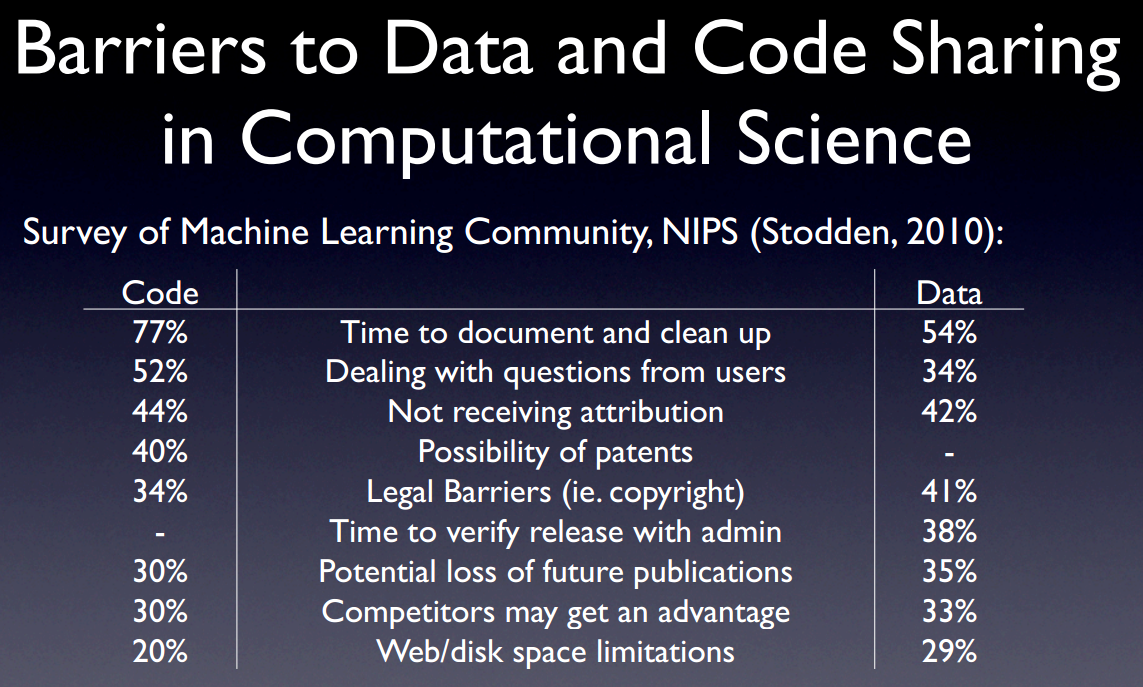
\includegraphics[width=\textwidth]{images/barriers}
\end{center}
}

\frame<1-2>[label=irreproducible]{
    \frametitle{Why is research still irreproducible?}
    \begin{enumerate}\itemsep2em
        \item<2-> Technology
        \item<3-> Individual actions
        \item<4-> Collective behavior and norms
    \end{enumerate}
}


\frame{
\begin{center}
    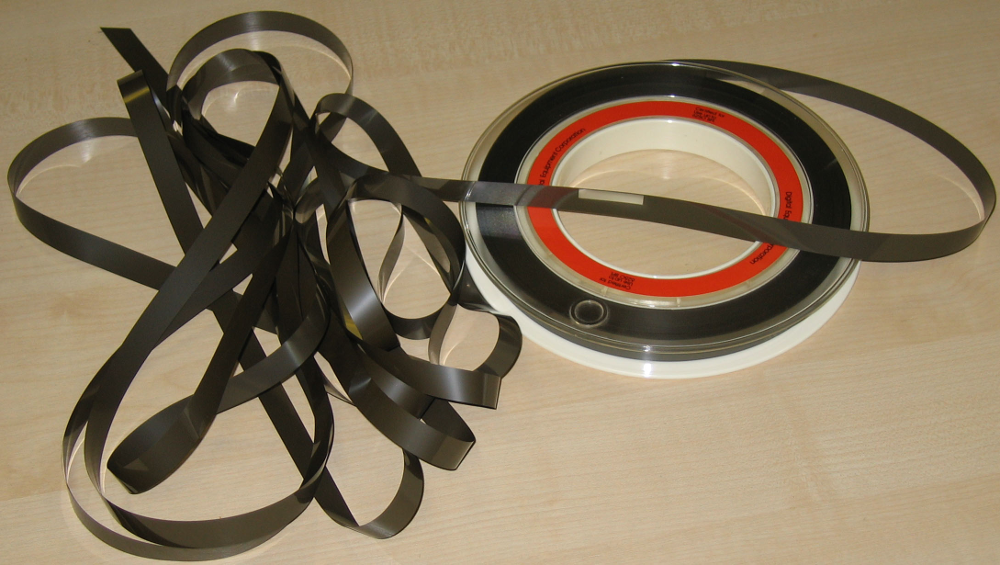
\includegraphics[width=\textwidth]{images/computertape} % http://commons.wikimedia.org/wiki/File:Tapesticker.jpg
\end{center}
}

\againframe<2->{irreproducible}


\section{What?}
\frame{\tableofcontents[currentsection]}

\frame<1-3>[label=what]{
    \frametitle{So what is reproducible research?}
    \begin{itemize}\itemsep2em
        \item<2-> Evolving standards and technology
        \item<3-> Discipline-specific meaning
        \item<4-> Hard to define
    \end{itemize}
}


\frame{
    \frametitle{American Association for Public Opinion Research\footnote[frame]{\href{http://www.aapor.org/disclosure_standards1.htm}{``Disclosure Standards''}}}
    Researchers must publish:
    \begin{enumerate}\itemsep1em
    	\item Research sponsor
    	\item Question wordings
    	\item Population, sampling frame, and sampling desng
    	\item Sample sizes and margins of error
    	\item Dates of data collection
    \end{enumerate}
}


\frame{
    \frametitle{American Psychological Assoc.\footnote[frame]{\href{http://www.apa.org/ethics/code/index.aspx}{``Ethical Principles of Psychologists and Code of Conduct''}}}
    \begin{itemize}
    	%\item ``Psychologists create, and to the extent the records are under their control, maintain, disseminate, store, retain and dispose of records and data relating to their professional and scientific work in order to (1) facilitate provision of services later by them or by other professionals, (2) allow for replication of research design and analyses, (3) meet institutional requirements, (4) ensure accuracy of billing and payments, and (5) ensure compliance with law.'' (6.01)
    	\item ``After research results are published, \textbf{psychologists do not withhold the data on which their conclusions are based from other competent professionals who seek to verify the substantive claims through reanalysis and who intend to use such data only for that purpose}, provided that the confidentiality of the participants can be protected and unless legal rights concerning proprietary data preclude their release\dots'' (8.14a)
    	%\item ``Psychologists who request data from other psychologists to verify the substantive claims through reanalysis may use shared data only for the declared purpose. Requesting psychologists obtain prior written agreement for all other uses of the data.'' (8.14b)
    \end{itemize}
}

\frame{
    \frametitle{Assoc. for Psychological Science\footnote[frame]{\href{http://www.psychologicalscience.org/index.php/publications/journals/psychological\_science/ps-submissions\#DISC}{``Submission Guidelines''}}}
    \begin{enumerate}\itemsep2em
    	\item Sample sizes and exclusion criteria
    	\item Report all manipulations used
    	\item Report all outcomes analyzed
    \end{enumerate}
}

\frame{
    \frametitle{American Anthropological Association\footnote[frame]{\href{http://www.aaanet.org/issues/policy-advocacy/upload/AAA-Ethics-Code-2009.pdf}{``Code of Ethics''}}}
    \begin{itemize}
    	\item ``Anthropological researchers should seriously consider all reasonable requests for access to their data and other research materials for purposes of research. They should also make every effort to insure preservation of their fieldwork data for use by posterity.''
    \end{itemize}
}

\frame{
    \frametitle{CONSORT Group\footnote[frame]{\href{http://www.consort-statement.org/consort-2010}{``CONSORT Statement''}}}
    \begin{itemize}
    	\item ``The checklist includes the 25 items selected because empirical evidence indicates that not reporting the information is associated with biased estimates of treatment effect, or because the information is essential to judge the reliability or relevance of the findings.''
    	\item No requirement for open data or analyses
    \end{itemize}
}


\frame{
	\frametitle{American Political Science Assoc.\footnote[frame]{\href{http://www.apsanet.org/Files/Publications/APSAEthicsGuide2012.pdf}{``A Guide to Professional Ethics in Political Science''}}}
	\begin{itemize}
		\item ``When statements that are challenged are based on reproducible data authors  are obliged to facilitate replication.'' (5.5)
		\item ``Researchers making evidence-based knowledge claims should reference the data they used to make those claims. If these are data they themselves generated or collected, researchers should provide access to those data or explain why they cannot.'' (5.6)
		\item ``Production transparency'' (6.2)
		\item ``Analytic transparency'' (6.3)
	\end{itemize}
}

\frame{
	\frametitle{European Research Council\footnote[frame]{\href{http://erc.europa.eu/sites/default/files/document/file/ERC\_Open\_Access\_Guidelines-revised\_2013.pdf}{``Open Access Guidelines for researchers funded by the ERC''}}}
	\begin{itemize}
		\item ``The European Research Council supports the basic principle of Open Access to research data. It therefore recommends to all its funded researchers that they follow best practice by retaining files of all the research data they have used during the course of their work, and that they be prepared to share this data with other researchers whenever it is not bound by copyright restrictions, by confidentiality agreements, or by contractual clauses.''
	\end{itemize}
}



\frame{
    \frametitle{PLoS\footnote[frame]{\href{http://www.plosone.org/static/policies.action\#sharing}{``Editorial and Publishing Policies''}}}
    \begin{itemize}\itemsep2em
    	\item ``Publication is conditional upon the agreement of the authors to make freely available any materials and information described in their publication that may be reasonably requested by others.''
    	\item Software created for use in publications must be open source
    \end{itemize}
}

\againframe<3-4>{what}


\frame{
    \frametitle{\textit{Ir}reproducibility}
    \begin{itemize}\itemsep0.25em
        \item<2-> Fabrication
        \item<3-> Human error
        \item<4-> Lack of methodological transparency
        \item<5-> Ambiguous data citations
        \item<6-> Proprietary data and file formats
        \item<7-> Unavailable data
        \item<8-> Analysis uses proprietary software/hardware
        \item<9-> Analysis unavailable
        \item<10-> ``Available from the author\only<11->{ (now deceased)}'' 
    \end{itemize}
}

\frame{
\begin{center}
    
\includegraphics[width=\textwidth]{images/bullshit}
\end{center}
}


\frame{
    \frametitle{Distinguish from other concepts}
    \begin{itemize}\itemsep3em
        \item<2-> \textit{Reproducible} versus \textit{Replicable}
        \item<3-> \textit{Reproducible} versus \textit{Automated}
        \item<4-> \textit{Reproducible} versus \textit{True}
    \end{itemize}
}


\frame{
    \frametitle{Arrive at a definition}
    Stanford University's David Donoho:
    \begin{center}
        \textit{``An article about computational science in a scientific publication is not the scholarship itself, it is merely advertising of the scholarship. The actual scholarship is the complete software development environment and the complete set of instructions which generated the figures.''}
    \end{center}
}

\frame{
    \Huge
    \begin{center}
        Reproducible research enumerates a complete set of physical actions needed to transforms transparent inputs into outputs.
    \end{center}
    % An article is not research, it is the output of research. Making an article reproducible (e.g., using knitr) is only part of a reproducible workflow.
}





\section{How?}
\frame{\tableofcontents[currentsection]}

\frame{
    \frametitle{What makes up the ideal reproducible research product?}
}

\frame{
    \begin{center}
        {\noindent\Large\visible<1>{\textbf{Past}} \hspace{2em} \visible<2>{\textbf{Present}} \hspace{2em} \visible<3>{\textbf{Future}}}
    \end{center}
    \only<1>{
    \begin{itemize}\itemsep2em
        \item Data and method description
        \item Closed data and analysis
        \item Use of proprietary software
        \item Paywalled publications
    \end{itemize}
    }
    \only<2>{
    \begin{itemize}\itemsep2em
        \item Detailed or full protocols
        \item Data and analysis sharing (on request)
        \item Mix of proprietary and open software
        \item ``Green'' open access
    \end{itemize}
    }
    \only<3>{
    \begin{itemize}\itemsep1em
        \item Study preregistration and ``outcome-blind'' review
        \item Open lab notebooks
        \item Persistent, archived, open-licensed data
        \item Open source software
        \item Open peer review
        \item Open access publication
        \item Literate, reproducible output
    \end{itemize}
    }
}






\frame{
    \frametitle{How do you make your work more reproducible?}
    \begin{center}
        \Huge
        \onslide<2>{Always think about your future self!}
    \end{center}
}

\frame{
	\begin{center}
		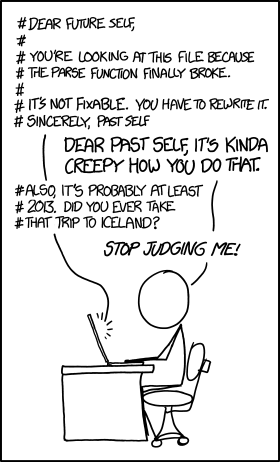
\includegraphics[height=.9\textheight]{images/futureself} % http://xkcd.com/1421/
	\end{center}
}




\frame<1>[label=notebook]{
    \frametitle{(1) Write Everything Down}
    \begin{enumerate}\itemsep2em
        \item<2-> Mark up your analysis files
        \item<3-> Write (and maintain) your research protocols
        \item<4-> Keep codebooks, questionnaires, and stimulus materials
        \item<5-> Try version control
    \end{enumerate}
}

\frame{
\begin{center}
    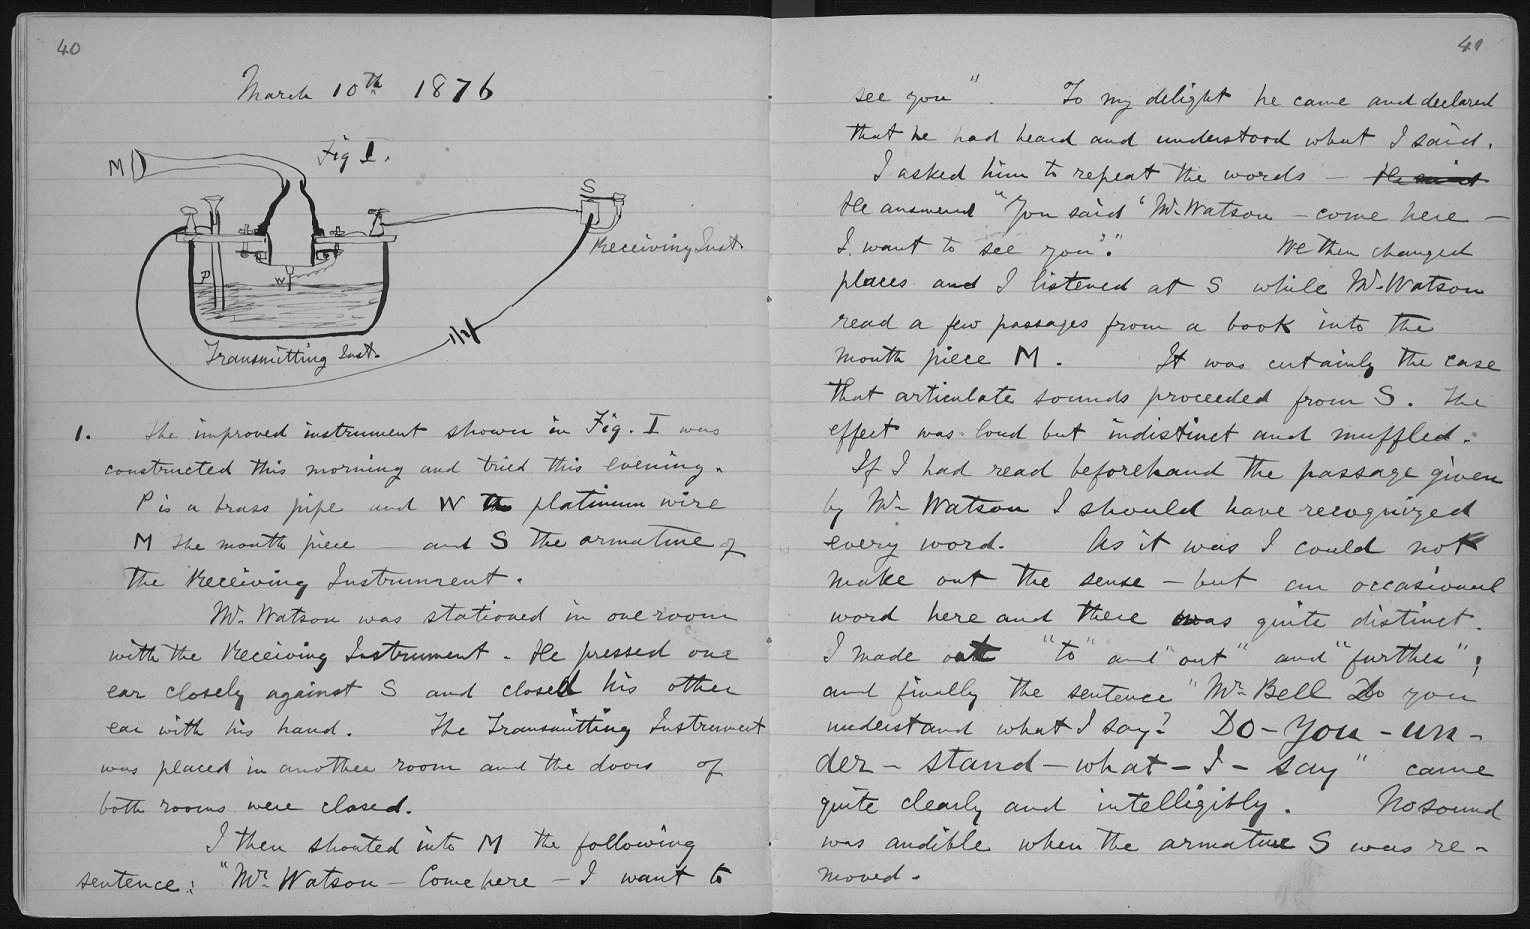
\includegraphics[width=\textwidth]{images/labnotebook}
\end{center}
}

\againframe{notebook}


\frame<1>[label=organized]{
    \frametitle{(2) Get Organized}
    \begin{enumerate}\itemsep2em
        \item<2-> Use a folder structure than can be shared
        \item<3-> Never use absolute file paths in code
    \end{enumerate}
}

\frame{
    \frametitle{My dissertation folder}
    \begin{center}
        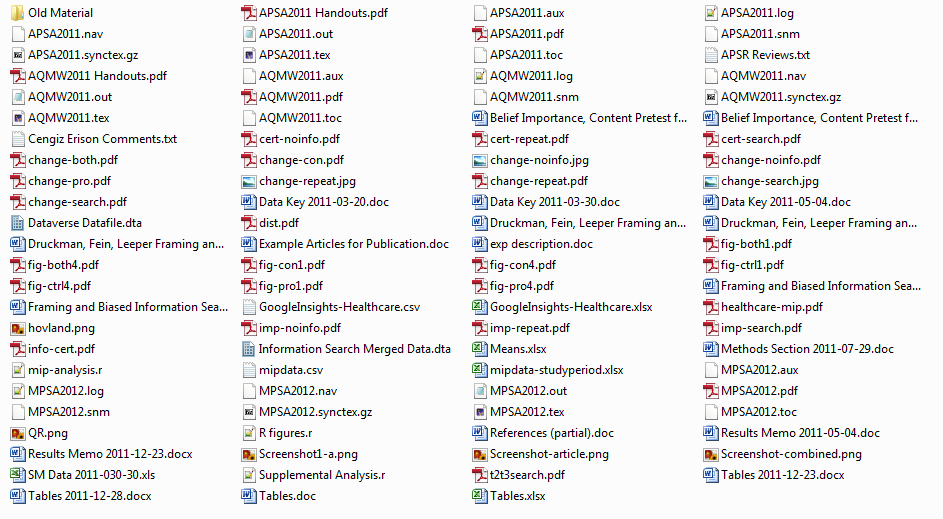
\includegraphics[width=\textwidth]{images/badfolder}
    \end{center}
}

\againframe<2>{organized}

\frame{
    \frametitle{Project Directory Structure}
    \begin{itemize}\itemsep0.5em
        \item Data
            \only<2>{
                \begin{itemize}
                    \item RawData.csv
                    \item CleanData.csv
                    \item Codebook.txt
                \end{itemize}
            }
        \item Analysis
            \only<3>{
                \begin{itemize}
                    \item GatherAndMerge.R
                    \item DataCleaning.R
                    \item Descriptives.R
                    \item Regression.R
                    \item Figures.R
                \end{itemize}
            }
        \item Figures
            \only<4>{
                \begin{itemize}
                    \item Distributions.png
                    \item MarginalEffects.png
                    \item PredictedValues.png
                \end{itemize}
            }
        \item Tables
            \only<5>{
                \begin{itemize}
                    \item Descriptives.tex
                    \item Regression.tex
                    \item MarginalEffects.tex
                \end{itemize}
            }
        \item Paper
            \only<6>{
                \begin{itemize}
                    \item Draft.tex
                    \item References.bib
                \end{itemize}
            }
        \item Presentation
            \only<7>{
                \begin{itemize}
                    \item Slides.tex
                \end{itemize}
            }
        \item Materials
            \only<8>{
                \begin{itemize}
                    \item Protocol.tex
                    \item StimulusMaterials.pdf
                    \item Questionnaire.txt
                \end{itemize}
            }
        \item README
    \end{itemize}
}

\frame{
    \begin{center}
        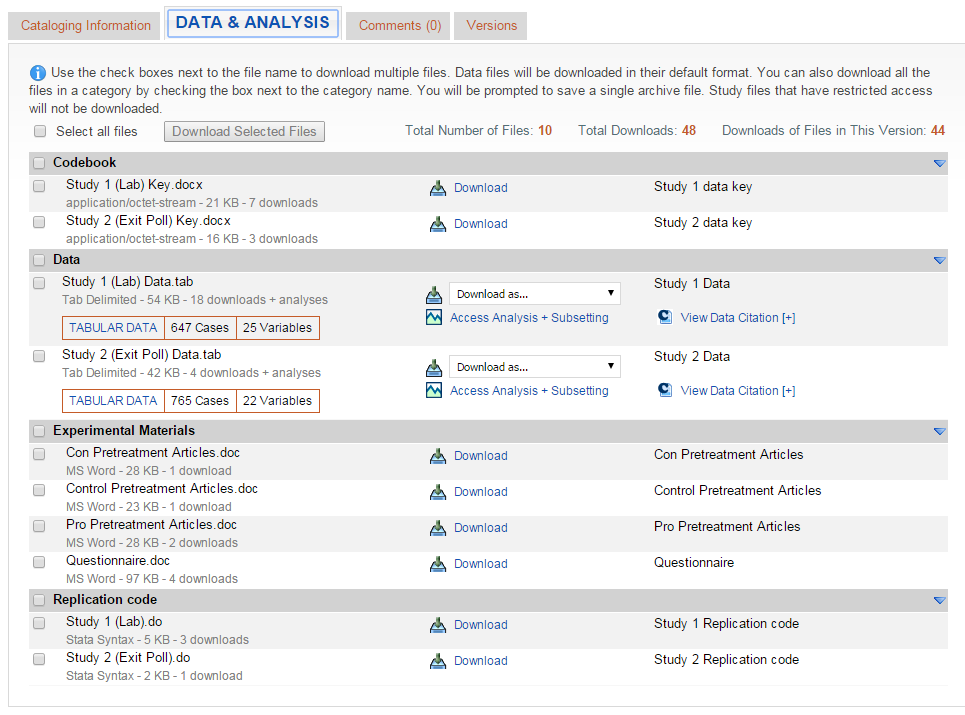
\includegraphics[width=\textwidth]{images/dataverseorganized}
    \end{center}
}

\againframe<3>{organized}


\frame{
\begin{center}
    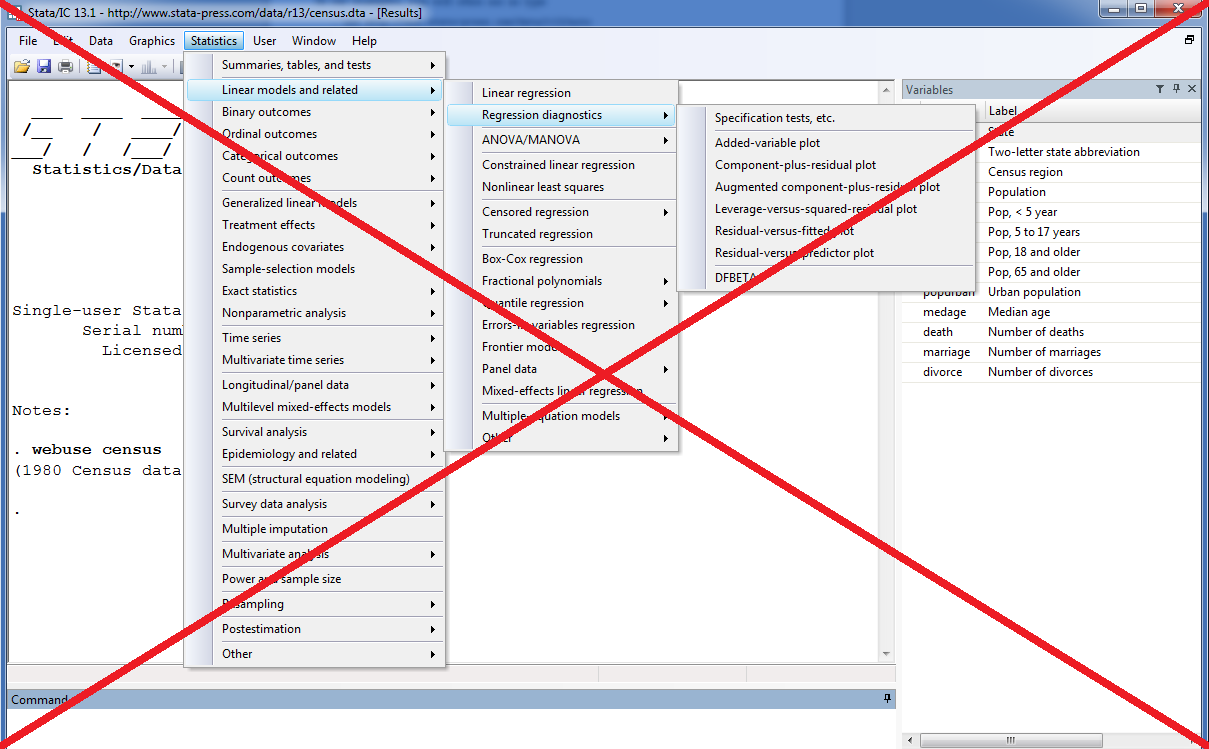
\includegraphics[width=\textwidth]{images/pointandclick}
\end{center}
}

\frame{
    \frametitle{(3) Abandon Point-and-Click}
    \begin{enumerate}\itemsep2em
        \item Don't clean data by hand
        \item Use scripts rather than menus for graphics
        \item Record your OS and software (and their versions)
    \end{enumerate}
}




\frame<1>[label=archive]{
    \frametitle{(4) Publicly Archive Your Research}
    \begin{enumerate}\itemsep2em
        \item<1-> Use persistent, public archives, not your website or ``on request''
        \item<2-> Use Simple, Structured, and Semantic open file formats
        \item<3-> Be explicit about data licensing
        \item<4-> Create useful metadata
    \end{enumerate}
}

\frame{
    \frametitle{Where do you archive your research?}
    \begin{itemize}\itemsep1.5em
        \item \href{http://thedata.org}{Dataverse Network}
        \item \href{http://datadryad.org}{Data Dryad}
        \item \href{http://figshare.com}{figshare}
    \end{itemize}
}


\againframe<2>{archive}

\frame{
\begin{center}
    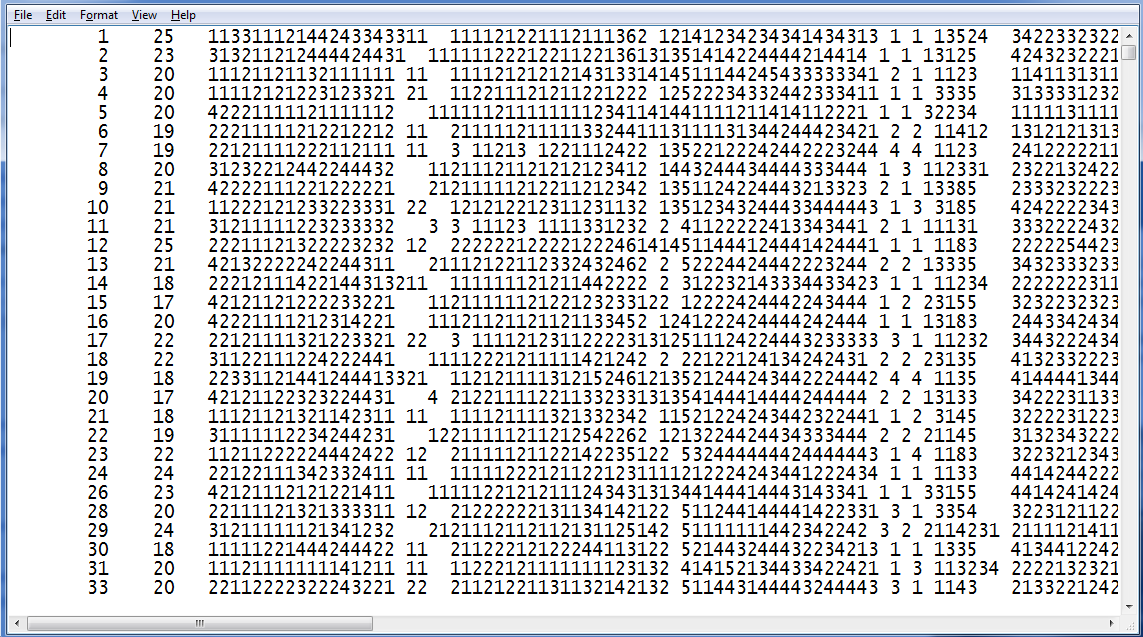
\includegraphics[width=\textwidth]{images/punchcarddata}
\end{center}
}

\frame{
\begin{center}
    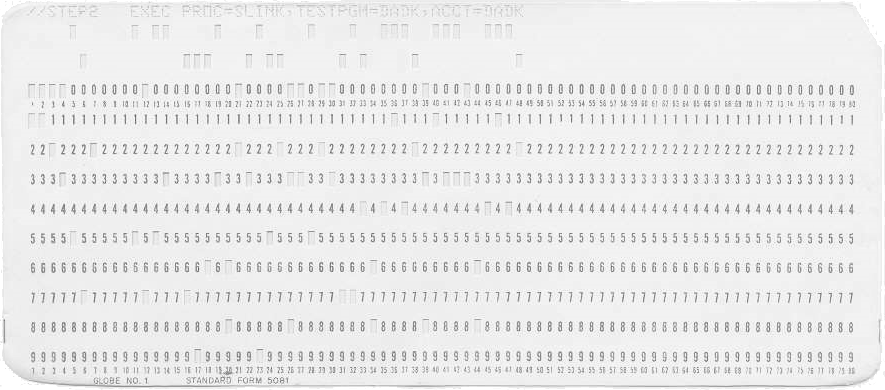
\includegraphics[width=\textwidth]{images/punchcard} % http://commons.wikimedia.org/wiki/File:Punch-card-5081.jpg
\end{center}
}

\frame{
\begin{center}
    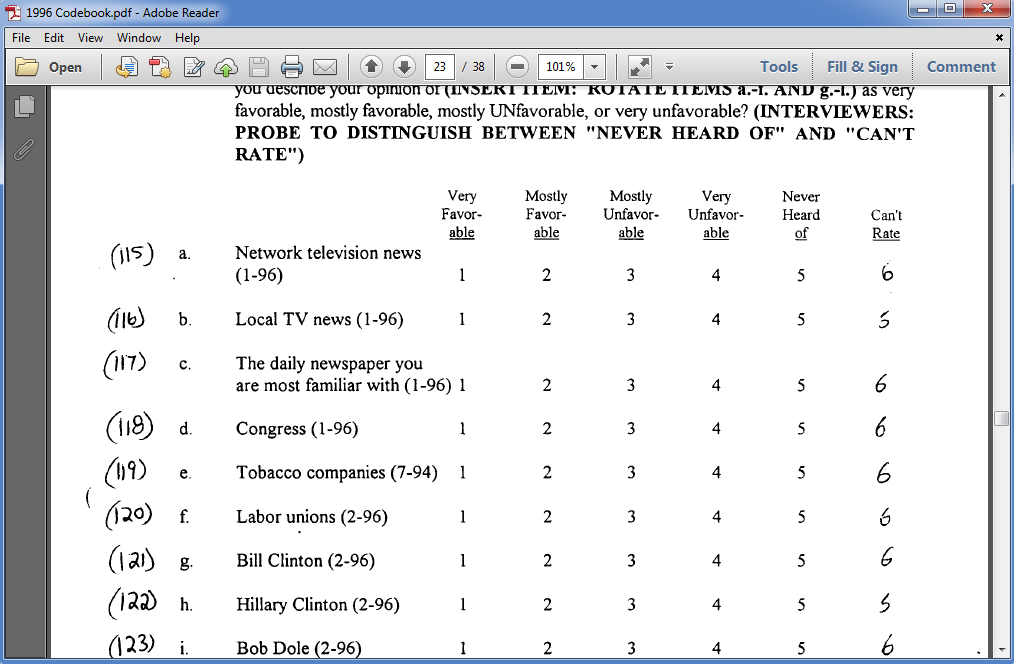
\includegraphics[width=\textwidth]{images/punchcardcodebook}
\end{center}
}


\againframe<3>{archive}


\frame{
    \frametitle{How to license data?}
    \begin{center}
        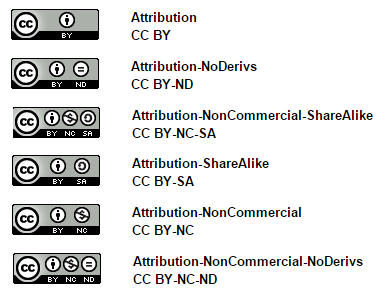
\includegraphics[width=.75\textwidth]{images/cclicenses}
    \end{center}
}



\againframe<4>{archive}




\frame{
    \frametitle{(5) Learn Literate Programming}
    \begin{columns}[c]
        \begin{column}{2in}
        
\includegraphics[width=\textwidth]{images/knitrlogo}
            % http://yihui.name/knitr/
        \end{column}
        \begin{column}{1in}
        \begin{center}
            \Huge{Learn to knit after lunch!}
        \end{center}        
        \end{column}
    \end{columns}
}



\frame{
    \frametitle{Where to go next?}
    \small
    \begin{itemize}
        \item \href{http://ropensci.org/blog/2014/06/09/reproducibility/}{rOpenSci}
        \item \href{http://www.nature.com/nature/focus/reproducibility/}{``Challenges in Irreproducible Research''}
        \item \href{http://kbroman.org/Tools4RR/pages/resources.html}{Karl Broman's resources} 
        \item \href{http://www.stodden.net/AMP2011/}{2011 ``Reproducible Research'' conference slides}
        \item \href{http://polmeth.wustl.edu/methodologist/tpm_v18_n2.pdf}{``Six steps to a Better Relationship with Your Future Self.''}
        \item \href{http://www.ploscompbiol.org/article/info\%3Adoi\%2F10.1371\%2Fjournal.pcbi.1003285}{``Ten Simple Rules for Reproducible Computational Research.''}
        \item \href{http://www.amazon.com/exec/obidos/ASIN/1466572841/7210-20}{\textit{Reproducible Research with R and RStudio}.}
        \item \href{http://software-carpentry.org/index.html}{Software Carpentry}
        \item \href{http://jhudatascience.org/}{Johns Hopkins Data Science Certificate on Coursera}
    \end{itemize}
}

\frame{
    \frametitle{People to follow?}
    \begin{itemize}\itemsep1em
        \item \href{https://twitter.com/victoriastodden}{@victoriastodden}
        \item \href{https://twitter.com/carlystrasser}{@carlystrasser}
        \item \href{https://twitter.com/l\_peer}{@l\_peer}
        \item \href{https://twitter.com/OSFramework}{@OSFramework} and \href{https://twitter.com/BrianNosek}{@BrianNosek}
        \item \href{https://twitter.com/RetractionWatch}{@RetractionWatch}
        \item \href{https://twitter.com/UCBITSS}{@UCBITSS}
        \item \href{https://twitter.com/openscience}{@OpenScience}
    \end{itemize}
}

\frame{
    \frametitle{Reproducibility isn't everything}
    \begin{itemize}\itemsep1em
        \item Data archiving and data citation
        \item Open protocols and materials
        \item Methodological transparency
        \item Free and open-source software (FOSS)
        \item Open access
    \end{itemize}
}




\section*{Conclusion}
\frame{\tableofcontents[currentsection]}

\frame{
    \frametitle{In the end\dots}
    \begin{itemize}\itemsep2em
        \item Be reproducible \textit{for you}
        \item Science will benefit as a result
    \end{itemize}
}


\appendix
\frame{}

\end{document}
